\section{Примеры}
\label{sec:samples}

%TODO для всех примеров. Привести к виду более похожему на тот, что в
%статье про пиксельные методы

Разберем примеры работы алгоритма на двух примерах. Но для начала
введем несколько дополнительных сущностей. Первая из которых это как
на практике будет выглядеть проверка условия корректности Фробениуса,
о котором упоминалось в \eqref{sec:csdisttrack}. Для этого введем
понятие скобки Ли (коммутатора) двух гладких вектор-функций $\varphi(x)$,
$\psi(x)$ одной и той же размерности $n$, являющихся столбцами матрицы $G(x)$


Пусть $\varphi_x$, $\psi_x$ --- $n \times n$ матрицы частных
производных функций $\varphi$ и $\psi$, а $x$ --- вектор размерности $n$. В примерах рассматриваем
матрицу $G(x)$ размерности $n=2$. В этом случае функция $\varphi_x$ к
примеру будет выглядеть так:
\begin{equation*}
  \begin{pmatrix}
    \frac{d \varphi_1}{d x_1} & \frac{d \varphi_1}{d x_2} \\
    \frac{d \varphi_2}{d x_1} & \frac{d \varphi_2}{d x_2}
  \end{pmatrix}(x)
\end{equation*}
Матрица $\psi_x$ --- выглядит аналогично. Тогда скобка Ли
$[\varphi,\psi]$ функций $\varphi$, $\psi$ определяется равенством.
\begin{equation*}
  [\varphi, \psi](x) = \varphi_x(x) \psi(x) - \psi_x(x) \varphi(x)
\end{equation*}
Очевидно, что она антикоммутативна т.е. $[\varphi, \psi] = - [\psi,
\varphi]$.

При условии того, что мы используем матрицу $2 \times 2$, мы будем
говорить, что рассматриваемая управляемая система удовлетворяет
условию корректности Фробениуса, если выполняется равенство

\begin{equation}
  \label{eq:1}
  [\varphi,\psi](x) \equiv 0.
\end{equation}

Второе о чем стоит поговорить это способ, благодаря которому мы
оцениваем порядок точности полученного результата --- между двумя множествами
вычисляется расстояние Хаусдорфа \eqref{eq:hausd_dist}.

\subsection{Пример системы без дрейфа}
\label{sec:snwd}

Сформулируем условия рассматриваемого примера

\begin{equation*}
  \begin{aligned}[b]
    &\dot{x_1}(t) = (1 -x_2(t))v_1(t), & x_1(0)=0\\
    &\dot{x_2}(t) = (1-x_1(t))v_2(t), & x_2(0) = 0\\[8pt]
    &v_1(t) \ge 0, v_2(t) \ge 0 \\
    &\int_{0}^{1} |v_1(t)| + |v_2(t)| dt \le V
  \end{aligned}
\end{equation*}


Стоит отметить, что для этой системы не выполнено условие корректности
Фробениуса (равенства нулю коммутатора). Покажем это. Возмем скобку
Ли (коммутатор) от двух гладких вектор-функций $\varphi$ и $\psi$,
являющимися столбцами матрицы

\begin{equation*}
  \begin{aligned}[b]
    G(x) = 
    \begin{pmatrix}
      \varphi & \psi
    \end{pmatrix},
    &
    \varphi =
    \begin{pmatrix}
      \varphi_1\\ \varphi_2
    \end{pmatrix},
    &
    \psi =
    \begin{pmatrix}
      \psi_1 \\ \psi_2
    \end{pmatrix}
  \end{aligned}
\end{equation*}


Скобка Ли тогда примет иметь вид ---

\begin{equation*}
  [\varphi,\psi] = \varphi_x \psi - \psi_x \varphi = 
  \begin{pmatrix}
    \frac{d \varphi_1}{d x_1} & \frac{d \varphi_1}{d x_2} \\
    \frac{d \varphi_2}{d x_1} & \frac{d \varphi_2}{d x_2}
  \end{pmatrix}
  \begin{pmatrix}
    \psi_1 \\ \psi_2
  \end{pmatrix}
  -
  \begin{pmatrix}
    \frac{d \psi_1}{d x_1} & \frac{d \psi_1}{d x_2} \\
    \frac{d \psi_2}{d x_1} & \frac{d \psi_2}{d x_2}
  \end{pmatrix}
  \begin{pmatrix}
    \varphi_1 \\ \varphi_2
  \end{pmatrix}
\end{equation*}

В этом примере матрица $G(x)$ имеет вид 

\begin{equation*}
  G(x) = 
  \begin{pmatrix}
    (1-x_2) & 0 \\
    0 & (1-x_1)
  \end{pmatrix}
\end{equation*}
В результмате несложных расчетов можно убедится, что условие корректности здесь не выполняется:
\begin{equation*}
  [\varphi,\psi] = 
  \begin{pmatrix}
    x_1 - 1\\
    x_2 - 1
  \end{pmatrix}
  \neq 0
\end{equation*}


Для этой системы была аналитически вычислена граница множества
достижимости в работе на основе работы \cite{AVS2016} Для разных
значений $V$ граница опиcывается немного по разному, но общий вид
формул отсается неизменным. На графиках линией обозначена граница
множества достижимости полученная аналитически и имеют вид

\begin{equation*}
  \begin{aligned}[b]
    &\Gamma^V_1 = \{ (1 - e^{-\frac{a}{2}},1 -
    e^{-\frac{a}{2}}+(V-a)e^{-\frac{a}{2}}), \quad a\in[0;V] \}\\
    &\Gamma^V_2 = \{ (1 -
    e^{-\frac{a}{2}}+(V-a)e^{-\frac{a}{2}},1 - e^{-\frac{a}{2}}),\quad
    a\in[0;V] \}\\
    &\Gamma^V_3 = \{a,(1-a)(V-a), \quad a\in[0;V] \}\\
    &\Gamma^V_4 = \{a,(1-a)(V-a), \quad a\in[0;V] \}
  \end{aligned}
\end{equation*}

А для $V \ge 2$ появляются еще линии

\begin{equation*}
  \begin{aligned}[b]
    &\Gamma^V_5 = \{ (1 - e^{\frac{a}{2}},1 +
    e^{\frac{a}{2}}+(V-2-a)e^{\frac{a}{2}}), \quad a\in[0;V-2]  \}\\
    &\Gamma^V_6 = \{ (1 -
    e^{\frac{a}{2}}-(V-2-a)e^{\frac{a}{2}},1 + e^{-\frac{a}{2}}), \quad a\in[0;V-2] \}\\
    &\Gamma^V_7 = \{ (1 +
    e^{\frac{a}{2}}+(V-2-a)e^{\frac{a}{2}},1 - e^{\frac{a}{2}}), \quad a\in[0;V-2] \}\\
    &\Gamma^V_8 = \{ (1 + e^{-\frac{a}{2}},1 -
    e^{\frac{a}{2}}-(V-2-a)e^{\frac{a}{2}}), \quad a\in[0;V-2] \}\\
  \end{aligned}
\end{equation*}


На Рис.~\ref{fig:v22} представлен пример множества достижимости 
\begin{figure}[h]
  \centering
  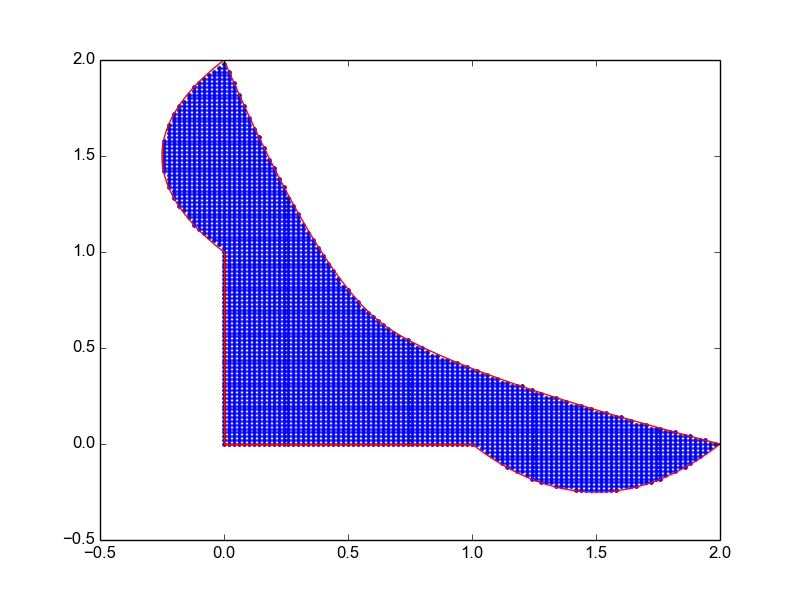
\includegraphics[width=0.5\linewidth]{img/figure_v_2_h_002.png}
  \hfil \caption{Множество достижимости для системы с V=2, h=0.02}
  \label{fig:v22}

\end{figure}

Для различных значений ресурса $V$ и шага сетки $h$ мы вычислили
расстояние хаусдорфа между теоретичесской оценкой множества
достижимости и тем, что получилось в результате работы
алгоритма. Результаты представлены в табл.~\ref{tab:hsd_ndft}, где в
первой колонке расположены значения ресурса $V$, во второй --- шага
$h$ и в третьей --- расстояния Хаусдорфа. Поскольку этот пример чисто
импульсный, здесь не приводится шаг по времени.Нетрудно заметить, что мы получаем линейный порядок сходимости в
зависимости от шага см рис.~\ref{fig:conv_nd}

\begin{table}[h]
  \centering
  \begin{tabular}{|*{3}{c|}}
    $V$&$h$&$\rho(A,B)$\\ \hline
    1&0.2&0.19357953184\\
    1&0.1&0.0989472244814\\
    1&0.04&0.04\\
    1&0.02&0.02\\
    1&0.01&0.01\\
    2&0.4&0.335023013171\\
    2&0.2&0.193935429287\\
    2&0.08&0.080131031276\\
    2&0.04&0.04\\
    2&0.02&0.02\\
    3&0.6&0.6\\
    3&0.3&0.29644979071\\
    3&0.12&0.130019551125\\
    3&0.06&0.0659015266245\\
    3&0.03&0.0309661912566\\
    5&1.0&1.14082938538\\
    5&0.5&0.5\\
    5&0.2&0.205052066625\\
    5&0.1&0.0985691231869\\
    5&0.05&0.0470656986497\\
    7&1.4&1.89238926658\\
    7&0.7&1.0191890624\\
    7&0.28&0.363069883153\\
    7&0.14&0.139983207703\\
    7&0.07&0.0724479673101\\
  \end{tabular}
  \caption{Расстояние Хаусдорфа в зависимости от шага сетки для
    различных значений ресурса}
  \label{tab:hsd_ndft}
\end{table}

\begin{figure}[h]
  \centering
  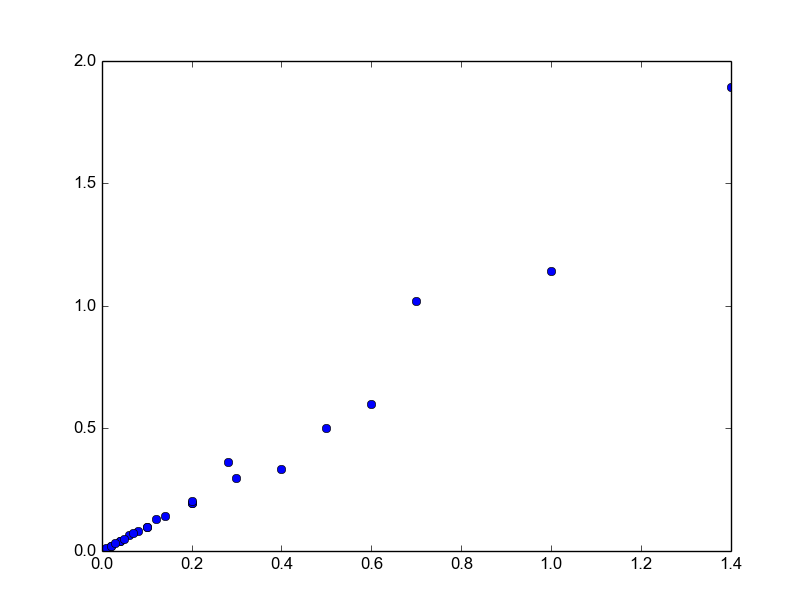
\includegraphics[width=0.5\linewidth]{img/conv_nd.png}
  \hfil \caption{Зависимость расстояния от шага сетки}
  \label{fig:conv_nd}
\end{figure}


\subsection{Пример системы с дрейфом}
\label{sec:swd}

В следующем примере, присутсвует простой дрейф. Для этого примера
также существует аналитическая оценка границы множества достижимости~\cite{AVS2016}

\begin{equation*}
  \begin{aligned}[b]
    &\dot{x_1}(t) = (1 -x_2(t))v_1(t), & x_1(0)=0\\
    &\dot{x_2}(t) = (1-x_1(t))v_2(t), & x_2(0) = 0\\[8pt]
    &v_1(t) \ge 0, v_2(t) \ge 0 \\
    &\int_{0}^{1} |v_1(t) + v_2(t)| dt \le V
  \end{aligned}
\end{equation*}

На Рис.~\ref{fig:h001_01} Представлено множество достижимости для
такой системы.

\begin{figure}[h]
  \centering
  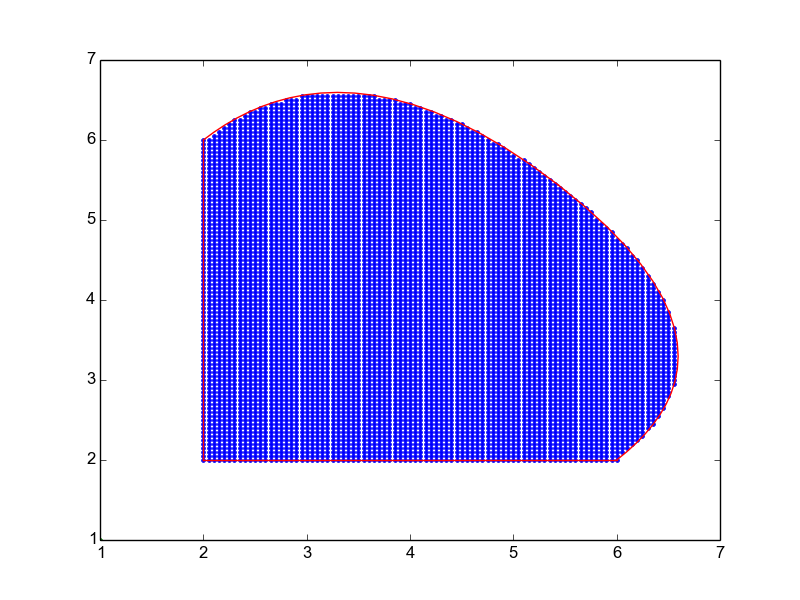
\includegraphics[width=0.5\linewidth]{img/figure_dc_h_005_ht_02}
  \hfil \caption{Множество достижимости для системы с h=0.05, ht=0.2}
  \label{fig:h001_01}
\end{figure}


В этой системе отклонение считалось для различных значений шага по
времени $h_t$ и шага сетки $h$. Мы вычислили
расстояние хаусдорфа между теоретичесской оценкой множества
достижимости и тем, что получилось в результате работы
алгоритма. Результаты представлены в табл.~\ref{tab:hsd_wdft}, где в
первой колонке расположены значения $h_t$, во второй --- шага
$h$ и в третьей --- расстояния Хаусдорфа. Нетрудно заметить, что здесь
мы также получаем линейный порядок сходимости в
зависимости от шага см рис.~\ref{fig:conv_d}


\begin{table}[h]
  \centering
  \begin{tabular}{|*{3}{c|}}
    $h_t$&$h$&$\rho(A,B)$\\ \hline
    1&0.2&0.217882468317\\
    1&0.1&0.1\\
    1&0.05&0.0474658824842\\
    1&0.01&0.00930483745156\\
    0.5&0.2&0.282842712475\\
    0.5&0.1&0.1\\
    0.5&0.05&0.0474658824842\\
    0.5&0.01&0.00930483745156\\
    0.2&0.2&0.217882468317\\
    0.2&0.1&0.1\\
    0.2&0.05&0.0474658824842\\
    0.2&0.01&0.00930483745156\\
    0.01&0.01&0.00930483745156\\
  \end{tabular}
  \caption{Расстояние Хаусдорфа в зависимости от шага сетки для
    различных значений ресурса}
  \label{tab:hsd_wdft}

\end{table}

\begin{figure}[h]
  \centering
  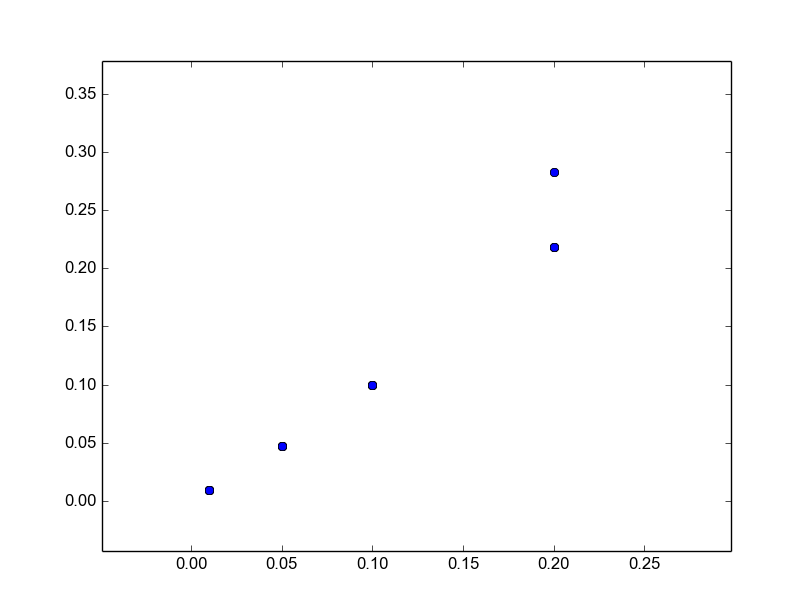
\includegraphics[width=0.5\linewidth]{img/conv_d.png}
  \hfil \caption{Зависимость расстояния от шага сетки}
  \label{fig:conv_d}
\end{figure}


\subsection{Пример без дрейфа с ограничением}
\label{sec:swdnrsb}
 
Данный пример также является чисто импульсным, как и первый, но с
одним введенными в систему дополнением --- матрица $G(x)$ умжножается
на $2 - x_1^2+ x_2^2$, таким образом система не должна выходить за
пределы круга радиуса $\sqrt{2}$.

\begin{figure}[h]
  \centering
  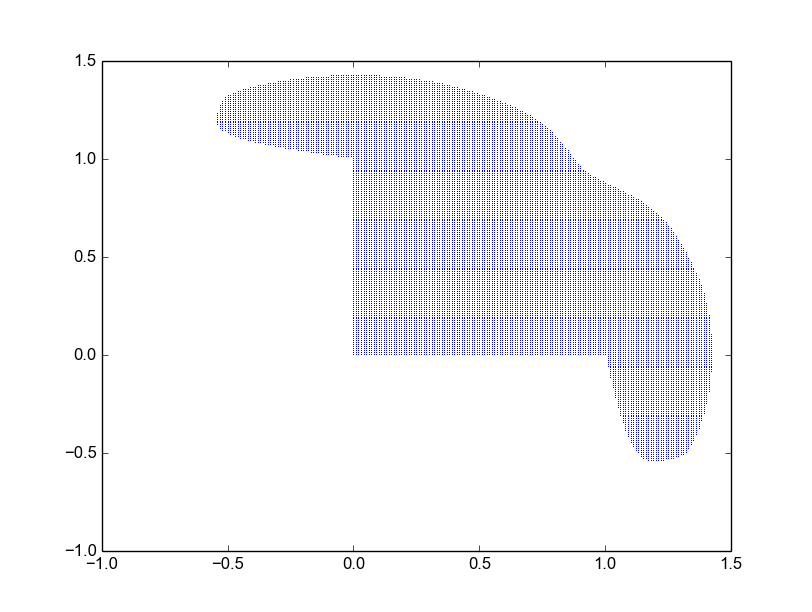
\includegraphics[width=0.5\linewidth]{img/figure_ndb_v7.png}
  \hfil \caption{Множество достижимости для системы с ограничением}
  \label{fig:vfb}
\end{figure}



\subsection{Пример с неодносвязным множеством достижимости}
\label{sec:swdnrs}


Интегральные кривые этого примера при нулевом управлении
представляют собой окружности с центром в начале координат, причем
фазовая скорость по модулю всюду равена 1. Как и в предыдущем примере,
управления неотрицательны.

\begin{equation*}
  \begin{aligned}[b]
    &\dot{x_1}(t) = \frac{x_2}{\left\|x\right\|} + x_1v_1, &x_1(0) =
    0,\quad v_1(t) \ge 0;\\
    &\dot{x_2}(t) = \frac{-x_1}{\left\|x\right\|} + x_2v_2, &x_2(0)
    = 0,\quad v_2(t) \ge 0.\\
    &\int\limits_0^{13} |v_1(t)| + |v_2(t)| dt \le 1
  \end{aligned}
\end{equation*}
Здесь $\left\| \cdot \right\|$ --- евклидова норма.

Для этого примера условие корректности
Фробениуса выполняется. 
В этом примере матрица $G(x)$ имеет вид 

\begin{equation*}
  G(x) = 
  \begin{pmatrix}
    x_1 & 0 \\
    0 & x_2
  \end{pmatrix}
\end{equation*}
И нетрудно убедиться, что здесь   $[\varphi,\psi] \equiv 0$

На Рис.~\ref{fig:v1h0.02} Представлено множество достижимости для
такой системы.


\begin{figure}[h]
  \centering

  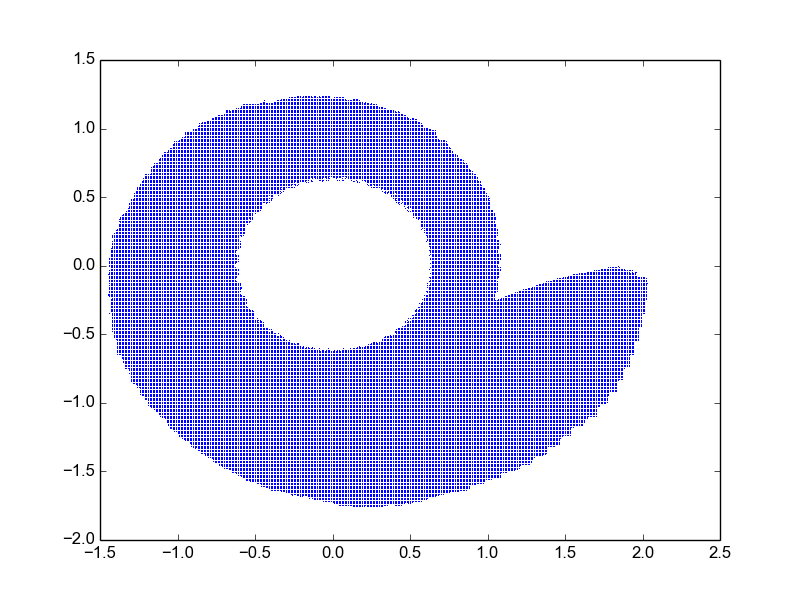
\includegraphics[width=0.5\linewidth]{img/figure_d_h_001_ht_01}
  \hfil \caption{Множество достижимости для системы с h=0.01, ht=0.1}
  \label{fig:v1h0.02}
\end{figure}


%%% Local Variables:
%%% mode: latex
%%% TeX-master: "rs-ids"
%%% End:
